\chapter{Entrenamiento y validación de los sistemas}
\label{chap:entrenamiento_y_validacion}

\nocite{aggarwal_recommender_2016}

% \begin{itemize}
%     \item En sistemas recomendadores, podemos distinguir dos paradigmas de evaluación~\cite{aggarwal_recommender_2016}:
%     \begin{itemize}
%         \item La evaluación online, en la que usuarios interactuan directamente con el \gls{sr} y se evalua como interactúan los usuarios con las recomendaciones presentadas
%         \item La evaluación offline con datos históricos, en la que se entrena un modelo utilizando interacciones previas de los usuarios (y tal vez otra información contextual).
%         \item La ventaja de usar un dataset offline es que se pueden comparar varios sistemas recomendadores, pero no conocemos como se comportarán en la realidad ni si se adaptarán a los cambios del conjunto de datos.
%         \item Obviamente, nuestro caso se tratará de una evaluación offline pues usamos datos históricos.
%         \item De todas formas, no podríamos hacer evaluación online utilizando solamente datos de la blockchain o las APIs públicas, necesitaríamos integrar el sistema en la plataforma.
%     \end{itemize}
%     \item Además, debido a la característica de los datos (cap~\ref{chap:problema}) no hay mucho escrito y ha habido que inventarse técnicas.
%     \item El objetivo es poder usar métricas clásicas de recsys como precision, ndcg o map, pero dividiendo los folds de manera temporal.
%     \item Por simplificar, asumimos que el tiempo es discreto, y que los modelos se entrenan periódicamente. Por ejemplo, cada día o cada semana, como se explica más en profundidad en el capítulo~\ref{chap:problema}.
%     \item En la siguiente sección se explorará como se ha realizado la división de los datos.
% \end{itemize}

En el ámbito de los sistemas recomendadores, existen dos paradigmas principales de evaluación~\cite{aggarwal_recommender_2016}. Por un lado, la \textit{evaluación online} utiliza la interacción directa de los usuarios con el sistema recomendador ya desplegado, permitiendo evaluar cómo responden los usuarios a las recomendaciones presentadas en tiempo real. Por otro lado, la \textit{evaluación offline} se basa en el uso de datos históricos, donde se entrena un modelo utilizando las interacciones previas de los usuarios, junto con cualquier información contextual disponible.

La ventaja de utilizar un dataset offline radica en la posibilidad de comparar varios sistemas recomendadores bajo condiciones controladas, aunque también sería posible utilizar A/B testing en una evaluación online para probar distintos modelos, asignando modelos distintos a cada usuario. Sin embargo, es importante tener en cuenta que el enfoque offline no proporciona una visión completa de cómo se comportarán los sistemas en la realidad ni si serán capaces de adaptarse a los cambios en el conjunto de datos a lo largo del tiempo. En nuestro caso, debido a la disponibilidad de datos históricos, utilizaremos una evaluación offline para entrenar y validar nuestros sistemas recomendadores, pero añadiendo la variable temporal para hacer más robusta la validación de los modelos y evitar el \textit{data leakage}, un riesgo presente en la evaluación offline de sistemas recomendadores~\cite{ji_critical_2023}.

La realización de una evaluación online requeriría una integración más estrecha del sistema recomendador desarrollado en la plataforma, lo que podría no ser factible utilizando únicamente datos de la blockchain o las APIs públicas disponibles. Sin embargo, al ser software libre, podría realizarse un fork de alguna de las plataformas modificando su interfaz para añadir el sistema recomendador, o crear una extensión de navegador que efectúe las recomendaciones.

Además, debido a las características específicas de estos datos, como se detalla en el capítulo~\ref{ch:planteamiento-problema}, se ha tenido que desarrollar técnicas y enfoques adaptados a nuestro contexto, que tengan en cuenta que las propuestas están abiertas durante un tiempo limitado. El objetivo es emplear métricas clásicas de sistemas recomendadores, como precisión, \acrshort{ndcg} o \acrshort{map} para que sean más fácilmente interpretables, pero teniendo en cuenta la naturaleza temporal de nuestros datos.

\section{División del conjunto de datos}
\label{sec:division_datos}

% \begin{itemize}
    % \item Debido a que no hay nada escrito sobre recomendadores de ítems acotados en el tiempo, no hay nada estándar o extendido sobre como evaluarlos.
    % \item La idea es segmentar el dataset en dos conjuntos, uno para entrenamiento, y otro para evaluación. Además, queremos validar el modelo con varios conjuntos de datos, por lo que realizaremos una especie de validación cruzada, pero utilizando el timestamp de los votos.
    % \item En un principio, podríamos usar la clase \url{TimeSeriesSplit} de Scikit-learn~\cite{pedregosa_scikit-learn_2011}, en la que se divide el conjunto de datos en K intervalos con el mismo número de muestras, pero los datos se ordenan por un timestamp, y se cogen incrementalmente. Es decir, el segundo fold incluye para entrenamiento los folds del primero, y el tercero incluye los de los dos anteriores, etc.
    % \item En nuestro caso, en lugar de dividir en intervalos con el mismo número de muestras, como la distribución de actividad no es uniforme en el tiempo (véase la figura~\ref{fig:rolling_proposals}), dividimos de tal manera que el intervalo temporal siempre sea el mismo, por ejemplo 7 días.
    % \item De esta manera, el primer fold cuenta de entrenamiento con los datos de la primera semana, y testea con la segunda. El segundo cuenta con los datos de las dos primeras semanas y testea con la tercera, y así...
    % \item Además, casi todas las propuestas del conjunto de entrenamiento ya han sido cerradas, y no pueden ser recomendadas, por lo tanto, no tiene sentido calcular las métricas de evaluación en train.
    % \item De igual modo, no tiene sentido usar todas las interacciones de test, pues muchas propuestas aún no han sido creadas, no pueden tener votos, y no hay ninguna interacción que sirva para el entrenamiento.
%     \item Por esa razón, las métricas se calculan únicamente sobre las interacciones producidas en el conjunto de test en propuestas que ya estaban creadas en el intervalo de train. Es decir, el conjunto de test es filtrado para mantener solo las interacciones en propuestas ya creadas. La figura~\ref{fig:example-train-test} ilustra con un ejemplo este comportamiento.
%     \item Tras desarrollar este sistema, descubrí que \textcite{macedo_context-aware_2015} ya habían realizado un método similar para un sistema de recomendación de eventos, con la diferencia de añadir una cota inferior al conjunto de entrenamineto, tratándose de un descubrimiento independiente o redescrubrimiento. La principal diferencia es que \citeauthor{macedo_context-aware_2015} añaden también una cota inferior al conjunto de entrenamiento.
% \end{itemize}

La evaluación de sistemas recomendadores con elementos limitados en el tiempo presenta un desafío, ya que no existe una metodología estándar ampliamente aceptada para su evaluación.

La estrategia seguida para abordar este problema es dividir el conjunto de datos en dos partes distintas: una para el entrenamiento del modelo y otra para su evaluación. Sin embargo, dado que se busca validar el modelo con múltiples subconjuntos de datos, se implementará una variante de la validación cruzada temporal. En este enfoque, se utilizarán las marcas de tiempo asociadas a los votos para realizar una partición temporal del conjunto de datos.

Inicialmente, consideramos utilizar la clase \url{TimeSeriesSplit} de Scikit-learn~\cite{pedregosa_scikit-learn_2011} para la división del conjunto de datos. Esta clase ordena los datos por su marca temporal, y divide el conjunto en $K$ intervalos, cada uno con un número igual de muestras. Además, las particiones son incrementales, de tal manera que en la partición $k$-ésima se retorna el split $k+1$ como conjunto de test, pero todos los splits de 0 a $k$ para entrenamiento, siendo cada uno un superconjunto del anterior.

Sin embargo, en nuestro caso, la distribución de actividad no es uniforme en el tiempo, como se ilustra en la figura~\ref{fig:rolling_proposals}. Por lo tanto, optamos por una estrategia alternativa, en la que el número de elementos en cada fold no es necesariamente el mismo, pero el intervalo de tiempo entre particiones sí lo es, y manteniendo que cada conjunto de entrenamiento sea un superconjunto del anterior. De hecho, podemos identificar cada fold por la marca de tiempo que divide los dos conjuntos. Los votos realizados antes de ese momento $t$ pertenecerán a entrenamiento y los realizados posteriormente, a la evaluación, lo que en el campo de \textit{forecasting} se conoce como \textit{out-of-sample testing}~\cite{tashman_out--sample_2000}.

\begin{figure}[b!]
    \centering
    % \fbox{\parbox{.7\linewidth}{Aquí va una figura creada con \url{draw.io} en la que se muestre como se divide el conjunto de datos en train y test, dado un timsetamp. Las propuestas serán rectángulos alargados, que tendrán puntos de colores que simbolizarán el feedback. Los puntos de un color estarán en el conjunto de entrenamiento, y los puntos de otro color estarán en test. También habrá puntos en blanco que no estén en ninguno de los dos conjuntos. Debe haber mínimo: (i) una propuesta con feedback en train y en test (ii) una propuesta que pase un poco a test pero sin feedback, (iii) una propuesta que no salga de train pero con puntitos de train, (iv) una propuesta solo en test, con puntitos en blanco porque no estan en ninguno de los dos conjuntos.}}
    % 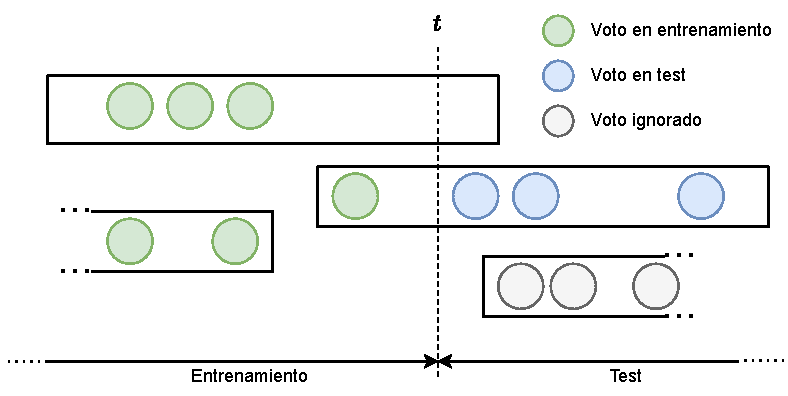
\includegraphics{figures/04_validacion/rs-time-folds-evaluacion.drawio.pdf}
    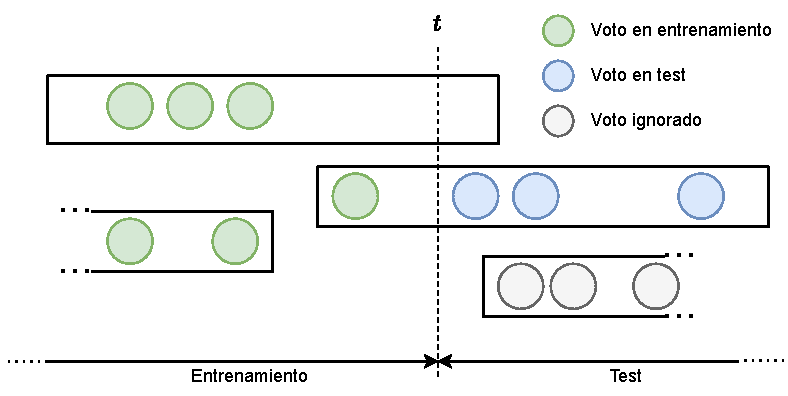
\includegraphics{figures/04_validacion/rs-time-folds-evaluacion.drawio.pdf}
    \caption[Esquema de la división en particiones de train y test.]{Esquema ejemplificando la creación de particiones de entrenamiento y test.}
    \label{fig:example-train-test}
\end{figure}

Además, es importante destacar que en el conjunto de entrenamiento, la mayoría de las propuestas ya han sido cerradas y, por lo tanto, no pueden ser objeto de recomendación pues los usuarios no podrían votar en ellas, aunque son útiles para crear el modelo del usuario.

De manera similar, al considerar el conjunto de prueba, nos encontramos con que muchas propuestas aún no han sido creadas y, como resultado, no habrán podido ser votadas por los usuarios durante el conjunto de entrenamiento y una predicción realizada sobre esas propuestas usando filtrado colaborativo carecerá de validez.
% Sin embargo, al tratarse de un problema de ranking, sí que se intentará recomendar esas propuestas que sólo aparecen en test. 
El recomendador basado en contenido sí que podrá realizar recomendaciones satisfactorias, mientras que el basado en filtrado colaborativo les asignará una prioridad mínima y probablemente no sean recomendadas. % Nótese que aunque sí podrían ser recomendadas basándose en el contexto y el contenido aunque no tengan aún votos, se ha decidido utilizar el mismo método de evaluación para los dos sistemas recomendadores desarrollados.

Por esa razón, las métricas se calculan exclusivamente utilizando las interacciones generadas en el conjunto de prueba en propuestas que ya estaban creadas durante el intervalo de entrenamiento. Es decir, el conjunto de prueba se filtra para conservar únicamente las interacciones en propuestas abiertas. La figura~\ref{fig:example-train-test} ejemplifica este procedimiento.

Tras desarrollar este sistema, se descubrió que~\textcite{macedo_context-aware_2015} ya habían implementado un método similar para un sistema de recomendación de eventos, aunque con la distinción de agregar un límite inferior al conjunto de entrenamiento. % Este hallazgo constituye un descubrimiento independiente o redescubrimiento.

Se ha implementado un código en Python para llevar a cabo este proceso, utilizando la tabla que contiene los votos y la que contiene las marcas de tiempo de las propuestas. Este código se encuentra en la función \url{timeFreqSplitCurrent}, ubicada en el módulo \url{src.model_selection}. Este módulo está disponible en el repositorio del proyecto en GitHub~\cite{davo_daviddavoupm-tfm-notebooks_2024}. Además, se incluye una versión simplificada del código en esta memoria, que se puede encontrar en Código~\ref{cod:timeFreqSplitCurrent}.

\begin{code}
%  \begin{minted}[breaklines]{python}
\begin{lstlisting}[language=Python]
def timeFreqSplit(dfv: pd.DataFrame, freq: str, dfp: pd.DataFrame, normalize=True):
  times = pd.date_range(dfv['timestamp'].min(), dfv['timestamp'].max(), 
                        freq=freq, normalize=normalize)
  for train_end in times[:-1]:
    train = df[df[timestamp_col] <= train_end]
    test = df[ (train_end < df['timestamp'])]
    
    open_proposals = dfp[ (dfp['start'] < train_end) & (train_end < dfp['end']) ]['id']
    test_filtered = test[test['itemID'].isin(open_proposals)]

    yield train, test_filtered
\end{lstlisting}
\caption{Simplificación del método \url{timeFreqSplit} del módulo \url{src.model_selection}}
\label{cod:timeFreqSplitCurrent}
\end{code}

Finalmente, para acomodar los datos al modelo LightGCN de Microsoft que necesita que los usuarios en test hayan estado previamente presentes en entrenamiento, se ignoran los votos de los usuarios nuevos: aquellos que aparecen tan sólo en el conjunto de test.

\subsection{Exploración de la división en folds de los datos de Decentraland}
\label{subsec:exploracion-folds}

% \begin{itemize}
%     \item En nuestro caso, para crear un sistema recomendador para Decentraland, se ha decidido dividir los folds en 7 días, debido a que es el tiempo de duración de las propuestas. Como contamos con datos de 2 años desde Mayo 2021 hasta Julio 2023, contamos con 112 folds con los que poder probar el sistema. En la figura~\ref{fig:04-first-ten-folds} se muestra el número de datos en entrenamiento y test de los 10 primeros folds.
%     \item Debido a restricciones computacionales, utilizamos solo los 10 últimos folds, con datos desde mayo hasta julio de 2023. Estos folds tienen entre 106~000 y 115~000 votos para el conjunto de entrenamiento (recordemos que son incrementales), y entre 13 y 25 propuestas en el conjunto de test, con una media de 381 votos de 123 usuarios con los que probar el modelo.
%     \item En un sistema de filtrado colaborativo, es necesario que las propuestas que vamos a recomendar tengan ya ciertos votos, pues, además de toda la historia incremental de votaciones que nos sirve para entrenar el modelo del usuario, es necesario saber qué tipos de usuarios han votado en una propuesta para recomendarla. En estos 10 folds, hay una media de 1283 votos por 325 usuarios en las propuestas que están abiertas en el momento de realizar el split y van a aparecer en la evaluación.
%     \item La tabla~\ref{tab:open_proposals} muestra más en profundidad los datos de cada uno de los 10 folds.
% \end{itemize}

Para desarrollar un sistema recomendador con los datos de la organización Decentraland, se ha optado por dividir los datos en folds de 7 días cada uno, pues es el período típico de duración de las propuestas dentro de la plataforma. Con los datos recopilados desde mayo 2021 hasta julio de 2023, se generan un total de 112 folds que podrían utilizarse para la evaluación del sistema. El conjunto de entrenamiento en estos folds es incremental, como se muestra en la figura~\ref{fig:04-first-ten-folds}.

\begin{figure}
    % No hace falta actualizarla porque en los primeros folds todas las propuestas eran de 7 días
    \centering
    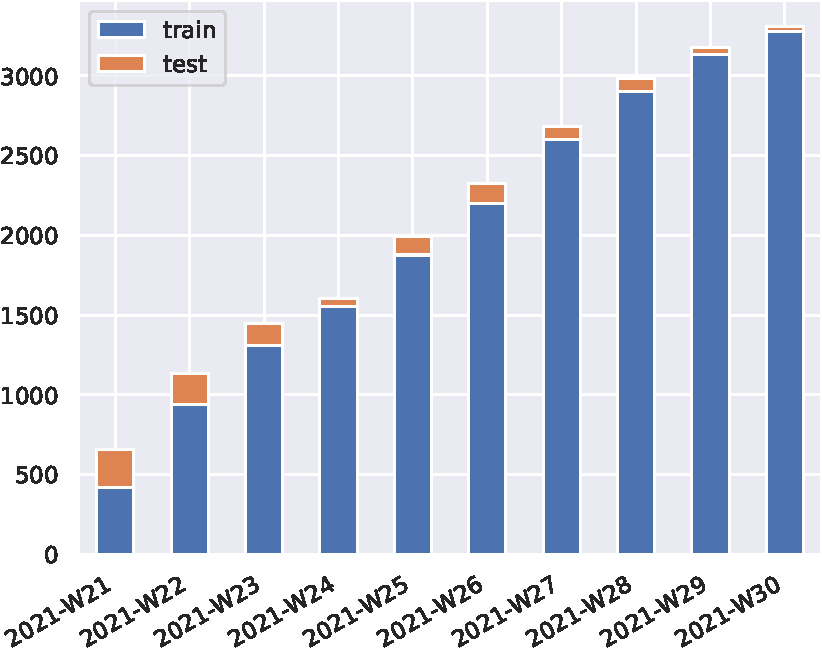
\includegraphics[width=.6\linewidth]{figures/04_validacion/10_first_folds_W-THU_True_Decentraland.pdf}
    \caption{Cantidad de votos en entrenamiento y prueba de los primeros 10 folds de la organización Decentraland.}
    \label{fig:04-first-ten-folds}
\end{figure}

% Source: 20_results.ipynb [9]
% Actualizado 2024-03-23
Sin embargo, por restricciones computacionales, se ha limitado el análisis a los 10 últimos folds, que abarcan desde mayo hasta julio de 2023. Estos folds contienen en entrenamiento casi todos los votos disponibles, yendo desde 106~000 a 115~000 votos. Por otro lado, el conjunto de test contiene una media de 439 votos de 142 usuarios realizados en entre 13 y 25 propuestas.

% No es necesario actualizar esto pues es en train
En un sistema de filtrado colaborativo, es fundamental que las propuestas a recomendar ya cuenten con cierta cantidad de votos para poder evaluarlas. Estas propuestas están abiertas en el momento de realizar el split, y aparecerán también en la evaluación. En estos 10 folds, hay una media de 1283 votos por 325 usuarios en dichas propuestas.

\begin{table}
    % Source: 20_results.ipynb [8]
    % Actualizado 2024-03-23
    \centering\footnotesize
    \begin{tabular}{l|r|rrrr|rrrr}
    \toprule
    \multicolumn{1}{c|}{\multirow{2}{*}{Semana}} &
    \multirow{2}{*}{\shortstack{Prop.\\ abiertas}} &
    \multicolumn{4}{c|}{\textbf{Solo entrenamiento}} &
    \multicolumn{4}{c}{\textbf{Solo validación}} \\
    \multicolumn{1}{c|}{} & & Votos & Usuarios & vpp & vpu & Votos & Usuarios & vpp & vpv \\
    \midrule
% 2023-W19 & 18 & 1627 & 358 & 90.39 & 4.54 & 322 & 130 & 17.89 & 2.48 \\
% 2023-W20 & 25 & 1346 & 305 & 53.84 & 4.41 & 713 & 147 & 28.52 & 4.85 \\
% 2023-W21 & 19 & 1483 & 305 & 78.05 & 4.86 & 296 & 108 & 15.58 & 2.74 \\
% 2023-W22 & 13 & 819 & 247 & 63.00 & 3.32 & 267 & 89 & 20.54 & 3.00 \\
% 2023-W23 & 13 & 631 & 191 & 48.54 & 3.30 & 291 & 94 & 22.38 & 3.10 \\
% 2023-W24 & 16 & 872 & 225 & 54.50 & 3.88 & 326 & 110 & 20.38 & 2.96 \\
% 2023-W25 & 17 & 1136 & 278 & 66.82 & 4.09 & 331 & 127 & 19.47 & 2.61 \\
% 2023-W26 & 10 & 838 & 278 & 83.80 & 3.01 & 204 & 92 & 20.40 & 2.22 \\
% 2023-W27 & 21 & 1591 & 469 & 75.76 & 3.39 & 683 & 198 & 32.52 & 3.45 \\
% 2023-W28 & 23 & 2493 & 600 & 108.39 & 4.16 & 382 & 141 & 16.61 & 2.71 \\
2023-W19 & 18 & 1627 & 358 & 90.39 & 4.54 & 354 & 139 & 19.67 & 2.55 \\
2023-W20 & 25 & 1346 & 305 & 53.84 & 4.41 & 811 & 169 & 32.44 & 4.80 \\
2023-W21 & 19 & 1483 & 305 & 78.05 & 4.86 & 332 & 122 & 17.47 & 2.72 \\
2023-W22 & 13 & 819 & 247 & 63.00 & 3.32 & 289 & 101 & 22.23 & 2.86 \\
2023-W23 & 13 & 631 & 191 & 48.54 & 3.30 & 341 & 118 & 26.23 & 2.89 \\
2023-W24 & 16 & 872 & 225 & 54.50 & 3.88 & 391 & 132 & 24.44 & 2.96 \\
2023-W25 & 17 & 1136 & 278 & 66.82 & 4.09 & 360 & 148 & 21.18 & 2.43 \\
2023-W26 & 10 & 838 & 278 & 83.80 & 3.01 & 239 & 107 & 23.90 & 2.23 \\
2023-W27 & 21 & 1591 & 469 & 75.76 & 3.39 & 890 & 249 & 42.38 & 3.57 \\
2023-W28 & 23 & 2493 & 600 & 108.39 & 4.16 & 384 & 142 & 16.70 & 2.70 \\
    \bottomrule
    \end{tabular}
    \caption{Número de propuestas abiertas en cada uno de los folds durante las últimas 10 semanas en Decentraland. Bajo \textit{Solo entrenamiento} se muestra el número de votos emitidos en esas propuestas que se han usado dentro del conjunto de entrenamiento, y los usuarios que han emitido esos votos. Un usuario puede haber votado en varias propuestas. A la derecha, bajo \textit{Solo validación} se muestra el número de votos emitidos en las propuestas durante la fase de validación. \textit{vpp} es el ratio de Votos Por Propuesta, y \textit{vpv} es el ratio de votos por Votante.}
    \label{tab:open_proposals}
\end{table}

En la tabla~\ref{tab:open_proposals} se muestra más en profundidad los datos de cada uno de los 10 folds, pero hay que destacar que los votos por cada votante en validación son en general muy bajos, a penas superando los 3 \gls{vpv} en dos de los folds.

% \begin{figure}
%     \centering
%     % \includegraphics{}
%     % \fbox{\parbox{.7\linewidth}{Aquí va un gráfico de barras que tiene en el eje X el fold actual, y en el eje Y el número de propuestas abiertas. Cada color de la barra es una DAO distinta. El problema de este gráfico es que si el número de propuestas abiertas es demasiado variable, o las diferencias entre las DAOs escogidas son muy grandes, entonces no servirá de nada.}}
%     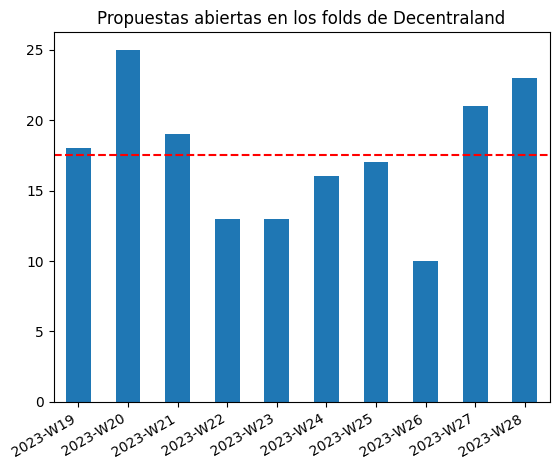
\includegraphics[width=10cm]{figures/04_validacion/propuestas_abiertas_decentraland.png}
%     \caption[Número de propuestas abiertas durante las últimas 10 semanas en Decentraland.]{Número de propuestas abiertas durante las últimas 10 semanas en Decentraland. Hubo una media (en rojo) de $17.5\pm4.72$ propuestas con las que verificar el modelo.}
%     \label{fig:open_proposals}
% \end{figure}

\section{Métricas utilizadas}
\label{subsec:metricas}

En esta sección se presentan métricas offline comúnmente empleadas en el ámbito de la recuperación de información y sistemas recomendadores. Se han utilizado las métricas disponibles en la librería Microsoft Recommenders~\cite{argyriou_microsoft_2020}.

\subsection{Precisión y exhaustividad}

\newcommand{\recall}[1]{recall@#1}
\newcommand{\precision}[1]{precision@#1}

% \begin{itemize}
%     \item Son métricas populares en la evaluación de sistemas recomendadores que han saltado del campo de la recuperación de información.
%     \item La precisión puede definirse como la probabilidad de que un ítem recuperado sea relevante, es decir el ratio entre el número de ítems relevantes recuperados y el número de ítems recuperados. 
%     \item La exhaustividad o \textit{recall} se define como la probabilidad de que un ítem seleccionado sea relevante, es decir, el ratio entre el número de ítems relevantes recuperados y el número total de ítems relevantes~\cite{herlocker_evaluating_2004}.
%     \item En un sistema recomendador que efectúa un ranking de los ítems a recomendar, podemos definir estas métricas dependiendo de los top $k$ items que elijamos recomendar, llamadas por su término en inglés $precision@k$ y $recall@k$. La fórmula de estas métricas se define en las ecuaciones \ref{eq:precision_at_k, eq:recall_at_k}.
%     \item El valor de estas métricas es muy dependiente de la $k$, por lo que no se pueden comparar métricas con distinto $k$.
%     \item Además, el mayor problema de estas métricas es que si el número de elementos relevantes es menor que $k$, como en nuestro caso, incluso un oráculo perfecto tendrá un valor menor que 1~\cite{manning_chapter_2008}.
% \end{itemize}

Las métricas de precisión y exhaustividad son ampliamente utilizadas en la evaluación de sistemas recomendadores, adoptadas desde el campo de la recuperación de información. La precisión se define como la probabilidad de que un ítem recuperado sea relevante, expresada como el cociente entre el número de ítems relevantes recuperados y el número total de ítems recuperados. Por otro lado, la exhaustividad, también conocida como recall, indica la probabilidad de que un ítem seleccionado sea relevante, calculada como el cociente entre el número de ítems relevantes recuperados y el número total de ítems relevantes~\cite{herlocker_evaluating_2004}.

En el contexto de un sistema recomendador que clasifica los ítems para su recomendación, estas métricas pueden ser adaptadas para evaluar únicamente los $k$ primeros ítems recomendados, conocidas como \textit{precisión en k} ($\precision{k}$) y \textit{exhaustividad en k} ($\recall{k}$). La fórmula de estas métricas se define en las siguientes ecuaciones:

\begin{minipage}{.5\textwidth}
    \begin{equation}\label{eq:precision_at_k}
        \precision{k} = \frac{|\text{items rel. rec. en $k$}|}{k}
    \end{equation}
\end{minipage}\begin{minipage}{.5\textwidth}
    \begin{equation}\label{eq:recall_at_k}
        \recall{k} = \frac{|\text{items rel. rec. en $k$}|}{|\text{items rel. en $k$}|}
    \end{equation}
\end{minipage}

Es importante tener en cuenta que el valor de estas métricas es altamente sensible al valor de $k$, por lo que no se pueden comparar métricas con distintos valores de $k$. Además, otro importante defecto de estas métricas ocurre cuando el número de elementos relevantes es menor que $k$, ya que incluso un sistema perfecto tendría un valor menor que 1 en estas métricas~\cite{manning_chapter_2008}.

Por esa razón, se consideró usar la métrica $r-precision$, la cual tiene en cuenta el número de documentos relevantes ($R$) para una consulta y calcula la precision en $R$ ($precision@R$), adaptando el valor de $k$ al número de documentos relevantes~\cite{manning_chapter_2008}. Como $k=R=\text{items rel. en k}$, esta métrica es equivalente al $recall@R$.

Sin embargo, a pesar de su potencial utilidad, no se empleó esta métrica debido a su ausencia en la librería Microsoft Recommenders~\cite{argyriou_microsoft_2020}. Su implementación requeriría tiempo adicional y podría afectar significativamente al tiempo de ejecución de la evaluación del modelo, y sus resultados están correlacionados con el \acrshort{map}, métrica que se explicará en la siguiente sección.

% \begin{itemize}
%     \item Por esa razón, se planteó el uso de la métrica $r-precisión$, que tiene en cuenta el número de documentos relevantes ($R$) para una query, y calcula la precisión en $R$ ($precision@R$), ajustando la $k$ al número de documentos relevantes~\cite{manning_chapter_2008}.
%     \item Como $k=R=\text{items rel. en k}$, esta métrica cumple la propiedad de que es también igual al $recall@R$.
%     \item Sin embargo, no se ha utilizado esta métrica debido a que al no estar dentro de la librería Microsoft Recommenders~\cite{argyriou_microsoft_2020}, habría que implementarla. Además, su implementación aumentaría notablemente el tiempo de evaluación del modelo.
% \end{itemize}

Finalmente, al evaluar el sistema recomendador al completo, para reportar una métrica se hace la media aritmética de el valor de dicha métrica para todos los usuarios a los que se les ha realizado una recomendación.

\subsection{Métricas de ranking}
\newcommand\DCG{\text{DCG}}
\newcommand\nDCG{\text{nDCG}}
\newcommand\IDCG{\text{IDCG}}
\newcommand\AveP{\text{AveP}}
\newcommand\MAP{\text{MAP}}
\newcommand\rel{\text{rel}}

Las métricas presentadas en la subsección anterior no tienen en cuenta el orden de las recomendaciones realizadas. Sin embargo, los modelos desarrollados sí que ordenan las recomendaciones, de manera que la primera recomendación para un usuario tiene un score superior o igual al del segundo (o pérdida menor).

Además, la lista de ítems recomendables para algunos usuarios es demasiado pequeña, por lo que conviene usar métricas que pongan más atención en las primeras o mejores recomendaciones, pero con una métrica agnóstica al modelo.

Se utilizarán las métricas \gls{ndcg} y \gls{map}, de uso extendido en \glspl{sr} e implementadas en la librería Microsoft Recommenders~\cite{argyriou_microsoft_2020}.

La \acrfull{dcg} de un usuario asigna un factor de descuento $log_2(i+1)$ al \textit{ranking} de cada ítem recomendado para ese usuario, y luego suma estos valores descontados para obtener una medida de la utilidad acumulada de las recomendaciones~\cite{aggarwal_recommender_2016}. Por lo general, en lugar de considerar todos los ítems, se calcula hasta un valor $k$ específico, similar a las métricas discutidas en la sección anterior. Así, la fórmula para el \gls{dcg} de un usuario se presenta en la ecuación~\ref{eq:dcg}. La \acrfull{ndcg} de cada usuario se calcula normalizando el \gls{dcg} obtenido con respecto al \gls{dcg} ideal (IDCG), y la fórmula está disponible en la ecuación~\ref{eq:ndcg}.

\begin{minipage}{.5\textwidth}
    \begin{equation}\label{eq:dcg}
        \DCG@k_u = \sum_{i=1}^{k} \frac{rel_i}{\log_2 (i+1)}
    \end{equation}
\end{minipage}\begin{minipage}{.5\textwidth}
    \begin{equation}\label{eq:ndcg}
        \nDCG@k_u = \frac{\DCG@k_u}{\IDCG@k_u}
    \end{equation}
\end{minipage}

Una vez normalizada, el rango del valor de esta métrica es de 0 a 1, lo que facilita su interpretación y permite comparar distintos modelos para un mismo conjunto de datos. Para calcular el \gls{ndcg} de un modelo dado, se obtiene la media de los \gls{ndcg} de cada usuario.

La relación entre precisión y exhaustividad (\textit{recall}) se puede representar mediante una curva de \textit{precision-recall}. La precisión media de un usuario ($\AveP$) se define como el valor medio de la precisión en esta curva. Y puede calcularse utilizando la siguiente suma finita~\cite{manning_chapter_2008}:

\begin{equation}
    \AveP@k = \frac{1}{k} \sum_{i=1}^k P(k)\cdot \rel(k)
\end{equation}

Aquí, $\rel$ indica la relevancia de la recomendación, que es 1 si estaba en el conjunto de prueba y 0 en caso contrario, tratándose de feedback implícito. La \acrfull{map} se obtiene realizando la media del $\AveP@k$ de todos los usuarios, y también tiene un valor entre 0 y 1.

% \begin{itemize}
    % \item Las métricas presentadas en la subsección anterior no tienen en cuenta el orden de las recomendaciones
    % \item Sin embargo, los modelos desarrollados en este trabajo sí que devuelven unas recomendaciones ordenadas, de tal manera que la primera recomendación para un usuario tiene un \textit{score} o \textit{pérdida} mejor o igual al del segundo
    % \item Además, debido a que la lista de items recomendables es tan pequeña, tiene sentido poner más atención en las mejores recomendaciones, aquellas de las que el sistema está \textit{más seguro}, pero con una métrica agnóstica al modelo, que no llegue a ser la función de pérdida y punto.
    % \item En la librería utilizada se implementan las métricas muy extendidas en la evaluación de \glspl{sr} llamadas \gls{ndcg} y \gls{map}.
    % \item La \gls{dcg} de un usuario asigna un factor de descuento $log_2(i+1)$ al ranking de cada item para cada usuario, y hace la suma del ranking descontado cada item recomendable. Normalmente, en lugar de utilizar todos los ítems, se calcula hasta un $k$ dado, al igual que en las métricas de la sección anterior, quedando el \gls{dcg} de un usuario con la siguiente fórmula ~\cite{aggarwal_recommender_2016}:

    % $$ \DCG@k_u = \sum_{i=1}^{k} \frac{rel_i}{\log_2 (i+1)}  $$

    % \item El \gls{ndcg} de cada usuario se calcula normalizando el \gls{dcg} obtenido con respecto al \gls{dcg} ideal (IDCG), tras ordenar los ítems relevantes por su relevancia.

    % $$ \nDCG@k_u = \frac{\DCG@k_u}{\IDCG@k_u} $$

    % \item Al estar normalizada, el rango del valor de esta métrica es de 0 a 1.
    % \item Finalmente, el \gls{ndcg} de un modelo dado se calcula haciendo la media de los \gls{ndcg} de cada usuario.
    
%     \item Puede expresarse la precisión como una función en base al recall, como una curva de precisión-recall.
%     \item La precisión media de un usuario ($\AveP$) es el valor medio de la precisión en esta curva, que puede calcularse con la siguiente suma finita~\cite{manning_chapter_2008}:
    
%     $$ \AveP@k = \frac{1}{k} \sum_{i=1}^k P(k)\cdot \rel(k) $$

%     \item Donde $\rel$ indica la relevancia de la recomendación, es decir, 1 si estaba en el conjunto de test, y 0 en caso contrario para feedback implícito.
%     \item La \acrfull{map} se calcula realizando el promedio de $\AveP@k$ de todos los usuarios.
%     \item Esta métrica también tiene un valor en el rango de 0 y 1.
% \end{itemize}


\section{Línea base}
\label{sec:linea_base}

Para desarrollar un sistema recomendador es esencial establecer una línea base para comparar entre modelos desarrollados. Esta línea base suele ser un algoritmo sencillo y sin personalización ni aprendizaje que proporciona un punto de referencia para comparar los resultados de los modelos. En este sistema recomendador, debido a la peculiar división en folds y los pocos elementos en test, los resultados de la evaluación son muy variables y dificultan la comparación entre los folds, siendo aún más necesaria esta línea base.

Una posible línea base pueden ser los resultados del estado del arte actual, si se tratase de un conjunto de datos extendido. En cualquier caso, la linea base debería ser un modelo establecido, pero debido a que no se han creado previamente sistemas recomendadores con estas características, es necesario introducir un nuevo modelo.

Una de las lineas base más simples, utilizada en el campo de la recuperación de información, consiste en realizar recomendaciones aleatorias entre los elementos recomendables, es decir, entre las propuestas abiertas, aunque esta linea base no proporciona un ranking y todas las recomendaciones tienen el mismo valor. 

Sin embargo, la línea base más extendida y ampliamente utilizada en \glspl{sr} es el modelo \textit{Más Populares} o \textit{MostPop}. Tampoco incorpora ningún nivel de personalización y simplemente recomienda los elementos con más interacciones registradas en el conjunto de datos. Esta linea base, además, destaca por su robustez, superando en ocasiones al filtrado colaborativo cuando los datos están altamente dispersos.

A pesar de su extensa popularidad, la implementación habitual de este modelo no siempre refleja fielmente la realidad~\cite{rendle_difficulty_2019}. Por ejemplo, no se considera la disponibilidad de los elementos en el momento de la recomendación, ni se tienen en cuenta la popularidad \textit{actual} de un ítem, recomendando en ocasiones elementos con los que un usuario no podría interactuar porque aún no están disponibles~\cite{ji_re-visit_2020}.

   % \item Es necesario tener un punto de referencia simple con el que comparar los otros modelos desarrollados con el mismo dataset. 
    % \item Además, debido a la peculiar división en folds, y los pocos elementos en test, los resultados de la evaluación son muy variables, y no pueden ser comparados entre sí.
    % \item Recordemos que el objetivo no es probar nuevos modelos, sino probar modelos existentes con este dataset, por lo que la línea base debería ser un modelo.
    % \item Debido a que el dataset no se ha utilizado nunca antes en sistemas recomendadores y no hay nada con lo que compararlo, es necesario utilizar un nuevo modelo como linea base.
    
    % \item La línea base más sencilla, usada en ocasiones en el campo de \gls{ir}, sería realizar recomendaciones aleatorias de entre los elementos recomendables.
    % \item Sin embargo, la línea base más extendida en \glspl{sr} es el modelo \acrfull{mp}, un modelo sin personaliozación que recomienda los items más populares (con más interacciones) del dataset.
    % \item Este modelo es muy robusto, superando en ocasiones el filtrado colaborativo cuando los datos son muy dispersos.
    % \item Como se recalca en \textcite{ji_re-visit_2020}, la implementación habitual de este modelo no es congruente con la realidad. Por ejemplo, no refleja los ítems que estaban disponibles en el momento, ni refleja la popularidad de los items en un instante según las interacciones realizadas, recomendando en ocasiones elementos con los que un usuario no podría interactuar porque aún no están disponibles, y por lo tanto realizando una subestimación.

\subsection{El modelo OpenPop}
\label{subsec:openpop}

El modelo desarrollado se denomina OpenPop y recomienda la propuesta abierta con más votos en un momento dado, siempre que el usuario aún no haya emitido su voto sobre ella. Esta estrategia se inspira en el modelo MostPop, y es similar al modelo RecentPop propuesto por \textcite{ji_re-visit_2020}, con la diferencia clave de que las propuestas, a diferencia de otros ítems, dejan de estar disponibles.

\begin{code}
%  \begin{minted}[breaklines]{python}
\begin{lstlisting}[language=Python]
import pandas as pd
from recommenders.datasets.pandas_df_utils import filter_by

def getBaselineRecommendations(train: pd.DataFrame, users, open_proposals, k: int = 5):
    # Number of votes in each proposal in train
    bestVotes = train[train['itemID'].isin(open_proposals)]['itemID'].value_counts()

    # Create pairs (userID, itemID) aka Microsoft's format
    df = pd.DataFrame(it.product(users, bestVotes.index), columns=['userID', 'itemID'])

    # Avoid recommending already voted proposals (they wont be in the test set)
    df = filter_by(df, train, ['userID', 'itemID'])

    # Get just top k recommendations (value_counts sorts by default)
    df = df.groupby('userID').head(k).reset_index(drop=True)

    df['prediction'] = True
    return df
\end{lstlisting}
\caption[Código del modelo OpenPop.]{Código del modelo OpenPop.}
\label{cod:openpop}
\end{code}

Desde el punto de vista de la implementación, dado un conjunto de datos de entrenamiento y prueba separados como se describe en la Sección~\ref{sec:division_datos}, el modelo simplemente cuenta el número de votos en el conjunto de entrenamiento para las propuestas abiertas, y elimina las recomendaciones que ya están presentes en el conjunto de entrenamiento. El código que implementa dicho modelo está en Código~\ref{cod:openpop}.

\subsection{Resultados de la línea base en Decentraland}

\begin{figure}[tb]
    \centering
    \begin{subfigure}{.48\textwidth}
        \centering
        % Source: 10_baseline_mp.ipynb [31]
        % Actualizado 2024-03-23
        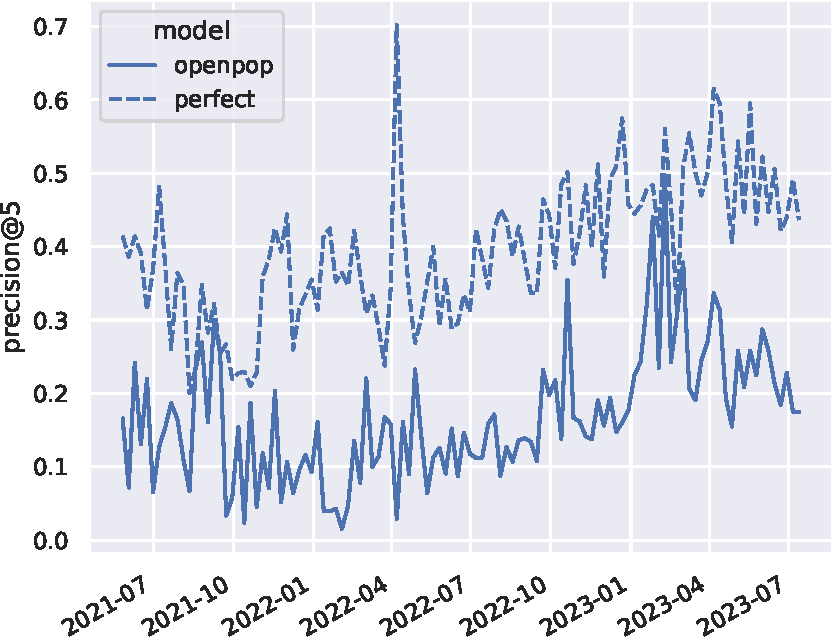
\includegraphics[width=\linewidth]{figures/04_validacion/10_all_precision@5_W-THU_True_Decentraland.pdf}
        \caption{Precisión en 5}
        \label{fig:openpop_precision@5}
    \end{subfigure}\hfill\begin{subfigure}{.48\textwidth}
        \centering
        % Source: 10_baseline_mp.ipynb [32]
        % Actualizado 2024-03-23
        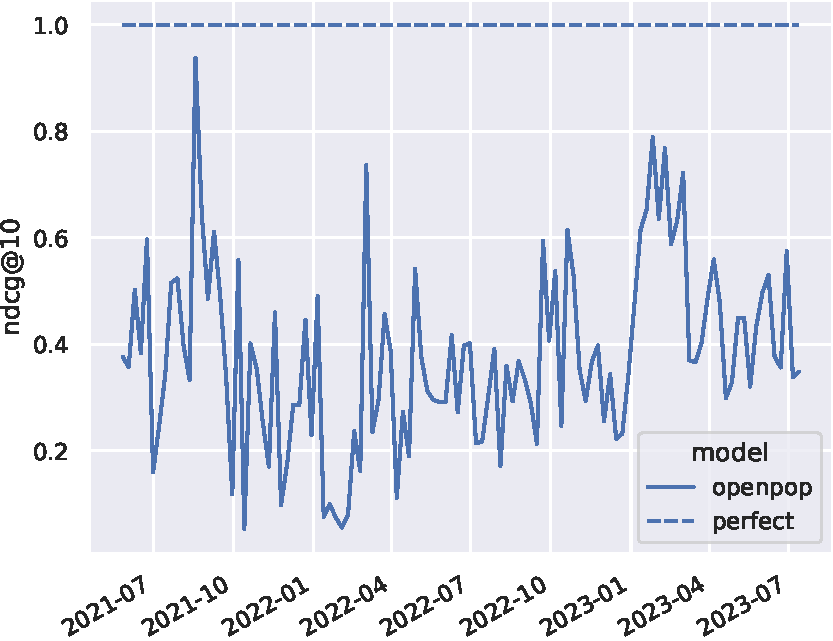
\includegraphics[width=\linewidth]{figures/04_validacion/10_all_ndcg@10_W-THU_True_Decentraland.pdf}
        \caption{nDCG en 10}
        \label{fig:openpop_ndcg@10}
    \end{subfigure}
    \caption[Resultados del modelo línea base.]{Resultados del modelo OpenPop (línea base) a lo largo de todos los folds disponibles.}
    \label{fig:openpop_results}
\end{figure}

Otra línea base utilizada, únicamente para compararlo con esta línea base, es el clasificador perfecto. Es necesario pues para algunas métricas utilizadas, al haber muy pocos votos disponibles en test por usuario, es imposible llegar a un valor de 1, como se explica en la sección~\ref{subsec:metricas}. Estos dos modelos y sus resultados se exploran en el \textit{notebook} \url{10_baseline_mp.ipynb} del repositorio del proyecto~\cite{davo_daviddavoupm-tfm-notebooks_2024}.


% Source: 10_baseline_mp.ipynb 
% Actualizado 2024-03-23
El análisis de los resultados del modelo OpenPop, utilizando la división de datos de la subsección~\ref{subsec:exploracion-folds}, revela una $\precision{5}$ media de $0.17\pm0.09$ en todos los folds. En comparación, un clasificador perfecto alcanza un valor de $0.39$, con un intervalo de confianza similar, lo que sugiere un amplio margen para mejorar el rendimiento del modelo. Esto indica que los usuarios no se limitan únicamente a las propuestas populares, e introducir personalización en las recomendaciones podría mejorarlas. Por otro lado, el valor medio del $\recall{5}$ es de $0.39\pm0.23$.

En términos de métricas de \textit{ranking}, el $\nDCG@10$ alcanza una media de $0.38\pm0.17$ a lo largo de todos los folds. Por definición, un clasificador perfecto obtendría un nDCG de 1. El $\MAP@10$ obtiene un valor de $0.28\pm0.16$.


La figura~\ref{fig:openpop_results} ilustra cómo la precisión, tanto en el caso perfecto como en la línea base, ha ido aumentando gradualmente con el tiempo, en paralelo al incremento de la participación. Sin embargo, el \gls{ndcg} es muy variable.

Es importante destacar que, para el entrenamiento y la validación de los modelos, se han utilizado exclusivamente los últimos 10 folds disponibles. En estos folds finales, la $\precision{5}$ de la línea base alcanza un valor de $0.22\pm0.04$ y la del modelo perfecto alcanza $0.47\pm0.06$, un valor significativamente más alto que en el resto de folds. Por su parte, el $\nDCG@10$ alcanza un valor de $0.42\pm0.09$, también mucho mejor.

% \begin{itemize}
%     % \item En todos los folds, el recomendador OpenPop consigue una $\precision{5}$ media de $0.17\pm0.09$, mientras que el clasificador perfecto consigue un valor de $0.39\pm0.09$, por lo que hay bastante hueco para mejora, dando a entender que los usuarios no se guían solo por las propuestas, y es necesario añadir personalización a las recomendaciones, aunque el modelo OpenPop no se queda atrás y es una línea base alta.
%     % \item El $\recall{5}$ medio es de $0.39\pm0.23$.
%     % \item En cuanto a métricas de ranking, el $\nDCG@10$ obtiene una media de $0.39\pm0.17$. El clasificador perfecto, por definición, tiene un \gls{ndcg} de 1. El $\MAP@10$ es de $0.28\pm 0.16$.
%     % \item Como se ve en la figura~\ref{fig:openpop_results}, la precisión, tanto perfecta como línea base, ha ido aumentando poco a poco, conforme a subido la participación a lo largo del tiempo. El \gls{ndcg}, sin embargo, es muy variable.
%     \item Sin embargo, como se especifica en la subsección~\ref{subsec:exploracion-folds}, para el entrenamiento y validación de los modelos solo se utilizan los últimos 10 folds disponibles. En estos últimos folds, la $\precision{5}$ base aumenta a $0.24\pm0.05$ con una $\precision{5}$ de $0.48\pm 0.06$ en el modelo perfecto. El $\nDCG@10$ es de $0.45\pm 0.09$.
% \end{itemize}


% \begin{itemize}
%     \item Dado un timestamp nuestro modelo baseline recomienda la propuesta abierta con más votos hasta el momento en la que el usuario aún no ha votado, y lo denominamos \acrfull{openpop}. Puede considerarse una modificación del modelo \textit{RecentPop} de \textcite{ji_re-visit_2020}, pero teniendo en cuenta el cierre de las propuestas.
%     \item A efectos de implementación, dado un conjunto de entrenamiento y test separados como se especifica en la sección~\ref{sec:division_datos}, simplemente es necesario contar el número de votos en entrenamiento de las propuestas abiertas, es decir, que están en ambos conjuntos.
% \end{itemize}

% \section{Entrenamiento de los modelos}
% \label{sec:entrenamiento_modelos}

% \begin{itemize}
%     \item En todos los casos se crea un nuevo modelo para cada fold, no se exprime nada del conocimiento aprendido.
%     \item Por esa razón
% \end{itemize}

% De esta manera, el modelo se ejecutará en intervalos discretos de tiempo, y la evaluación será en consecuencia. Es decir, asumiendo que el recomendador se ejecutará de forma periódica (por ejemplo, cada semana o cada día) y se evaluará de acuerdo con esta periodicidad. No se contempla la ejecución continua, sino que presupone la posibilidad de reentrenar completamente el modelo en cada ocasión que se desee realizar nuevas recomendaciones. Por consiguiente, uno de los requisitos es que el entrenamiento de los sistemas desarrollados sea rápido, con tiempos de entrenamiento en el orden de minutos.
